\documentclass{article}
\usepackage{caption}
\usepackage{amssymb}
%\usepackage{array}
\usepackage{geometry}
%\usepackage{scrextend}
\usepackage{amsmath}
%\usepackage{hyperref}
\usepackage{graphicx}
\usepackage{pdfpages}
%\usepackage{multicol}
\usepackage{tabularx}
\usepackage{float}

\title{EE102 Homework 2}
\author{Jacob Guenther}

\geometry{
	a4paper,
	total={170mm,257mm},
	left=20mm,
	top=20mm,
}

\graphicspath{{/home/jacob/}}

\begin{document}

\includepdf[pages=1,pagecommand={}]{Lab_2_cover.pdf}

\section{Objective}
\paragraph{}
The goal of this lab is to gain more experience using a multimeter while exploring some of the properties of a linear voltage regulator. In it we use a multimeter to measure node and differential voltage. Then we break the circuit to measure current. Finally simulate the circuit using OrCad and compare our measured results to the simulation.

\section{Equipment}
\begin{itemize}
	\item Agilent 34410A Multimeter
	\item Agilent E354xA Dual Output Power Supply
	\item 78L05 Linear Voltage Regulator
	\item 1k Resistor
	\item 1u Capacitor
	\item Prototyping Board
\end{itemize}

\section{Setup}
\paragraph{}
The circuit used in this lab is shown in figure 1. Node A is measured between the voltage source and ground. Node B is measured at the point between the regulator and the 1k resistor and ground. The differential voltage is measured at the input and output of the linear regulator. To measure the current through the 1k resistor the wire between the regulator and the resistor is removed and the probes are placed at the out leg of the regulator and one leg of the resistor.

\begin{figure}[H]
	\begin{center}
		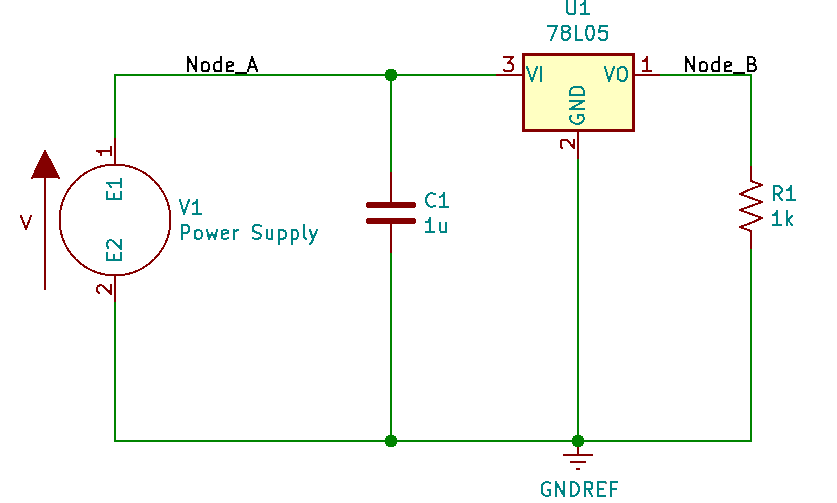
\includegraphics[width=10cm]{lab2schematic.png}
	\end{center}
	\caption{Schematic for the circuit used in this lab.}
\end{figure}

\section{Observations and Results}

\begin{table}[H]
\begin{tabularx}{\textwidth}{ | X | X | X | X | X | X | }
	\hline
	\textbf{Measured Node Voltage $\text{V}_\text{A}$} &
	\textbf{Measured Node Voltage $\text{V}_\text{B}$} &
	\textbf{Measured Differential Voltage $\text{V}_\text{AB}$} &
	\textbf{Measured Current Through 1 k$\Omega$} &
	\textbf{Calculated Differential Voltage $\text{V}_\text{A}-\text{V}_\text{B}$} &
	\textbf{Calculated Resistance} \\
	(V) & (V) & (V) & (mA) & (V) & ($\Omega$) \\
	\hline
	1.5 & 0.00020238 & 1.474 & 0.0015 & 1.5  & 134.92 \\
	2.0 & 0.669      & 1.329 & 0.661 & 1.331 & 1012.103  \\
	2.5 & 1.189      & 1.396 & 1.028 & 1.311 & 1156.615 \\
	3.0 & 1.611      & 1.380 & 1.589 & 1.389 & 1013.845 \\
	3.5 & 2.096      & 1.433 & 2.065 & 1.404 & 1015.012 \\
	4.0 & 2.583      & 1.439 & 2.545 & 1.417 & 1014.931 \\
	4.5 & 3.072      & 1.455 & 3.026 & 1.428 & 1015.202 \\
	5.0 & 3.563      & 1.470 & 3.510 & 1.437 & 1015.1 \\
	5.5 & 4.0563     & 1.531 & 3.993 & 1.444 & 1015.853 \\
	6.0 & 4.53       & 1.466 & 4.470 & 1.47  & 1013.423 \\
	6.5 & 4.924      & 1.574 & 4.860 & 1.576 & 1013.169 \\
	7.0 & 5.067      & 1.917 & 5.000 & 1.933 & 1013.4 \\
	7.5 & 5.069      & 2.435 & 5.014 & 2.431 & 1010.969 \\
	8.0 & 5.07       & 2.981 & 5.037 & 2.93  & 1006.552 \\
	8.5 & 5.066      & 3.316 & 5.058 & 3.434 & 1001.582 \\
	9.0 & 5.069      & 3.914 & 5.060 & 3.931 & 1001.778 \\
	\hline
\end{tabularx}
\caption{\label{tab:table-name}Displays the measured node and differential voltages, and current, as well as calculated differential voltage and resistance.}
\end{table}

\paragraph{}
To calculate the differential voltage we use the following equation.

\begin{equation}
	\text{V}_\text{AB} = \text{V}_\text{A} - \text{V}_\text{B}
\end{equation}

\paragraph{}
To calculate the expected resistance we use Ohm's Law, equation (2).

\begin{equation}
	\text{R} = {\text{V}_\text{B} \over \text{I}}
\end{equation}

\paragraph{}
Note that current is measured in mA so first we must convert it to amps to get our result in ohms.

\paragraph{}
One irregularity in the results can be seen when the input voltage was 1.5 volts. At this input the current was 0.0015 mA. This lead to the calculated resistance being 135 $\Omega$ far less than the 1 k$\Omega$ that is expected.

\paragraph{}
Next we run a simulation of the circuit using OrCad. The results of the simulation can be found in figures (1) and (2) plotted with my own measurements (figure 1) and with the rest of the classes measurements (figure 2). In figure 1 we can see that the measured results start aligning with the simulation around 3 volts. Between 1.5 and 3 volts the output is higher than expected. This could be because the model used for the regulator in the simulation is wrong, the process used to create the regulator has changed or is inconsistent, or because the regulator was hot from dissipating heat.

\begin{figure}[H]
	\begin{center}
		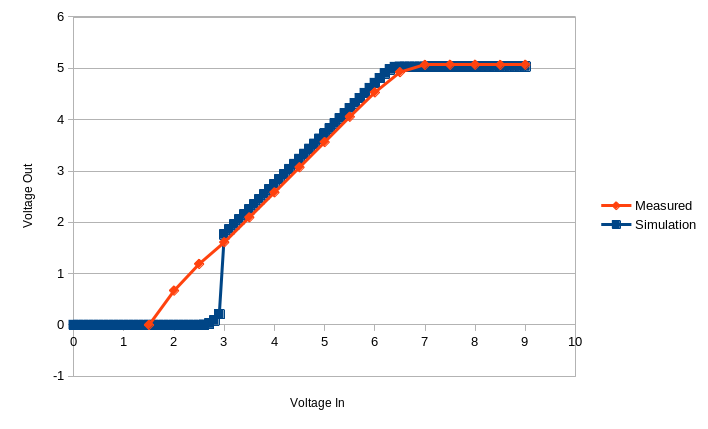
\includegraphics[width=\textwidth]{measured_chart.png}
	\end{center}
	\caption{Voltage Out vs Voltage In. Measured output voltage, and simulation output voltage.}
\end{figure}

\paragraph{}
In figure 2 we see that many of the measurements do not align with the expected output. I suspect the measurements that are still linear after 6.5 volts had the probes in the wrong place and/or had their circuits wired wrong. The measurements that that follow the curve but are higher than expected might not have nulled their multimeters.

\begin{figure}[H]
	\begin{center}
		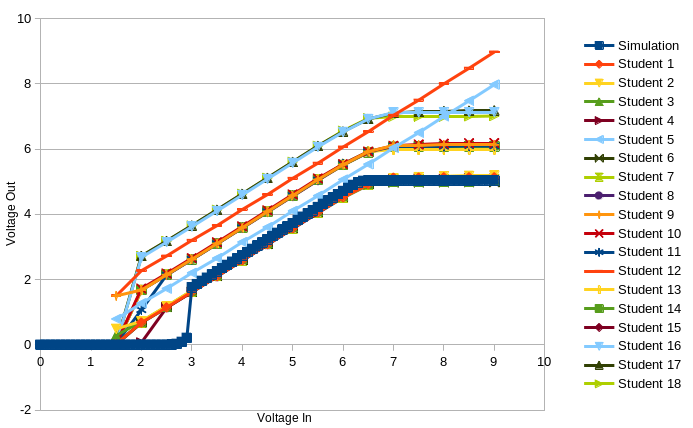
\includegraphics[width=\textwidth]{class_chart.png}
	\end{center}
	\caption{Voltage Out vs Voltage In. Classes measurements outputs and schematic simulation output.}
\end{figure}


\newpage
\section{Conclusion}
\paragraph{}
In this lab we used a multimeter to measure the input, output, and differential voltage across a linear regulator. We found that linear regulators are good when The input voltage is close to the output voltage, otherwise they dissipate lots of power in the form of heat.

\subsection{Sources of Error}

\begin{itemize}
	\item Temperature is not controlled for. Temperature can effect the efficiency of the device.
\end{itemize}


\newpage
\section{References}
\noindent
[1] Denise Thorsen, Maher Al-Badri, INTRODUCTION TO ELECTRICAL AND COMPUTER ENGINEERING, University of Alaska Fairbanks, 2022.
\newline
\newline
\noindent

\end{document}